\documentclass[a4paper,14pt]{extarticle}

\usepackage[utf8x]{inputenc}
\usepackage[T1,T2A]{fontenc}
\usepackage[russian]{babel}
\usepackage{hyperref}
\usepackage{indentfirst}
\usepackage{here}
\usepackage{array}
\usepackage{graphicx}
\usepackage{caption}
\usepackage{subcaption}
\usepackage{chngcntr}
\usepackage{amsmath}
\usepackage{amssymb}
\usepackage{pgfplots}
\usepackage{pgfplotstable}
\usepackage[left=2cm,right=2cm,top=2cm,bottom=2cm,bindingoffset=0cm]{geometry}
\usepackage{multicol}

\renewcommand{\le}{\ensuremath{\leqslant}}
\renewcommand{\leq}{\ensuremath{\leqslant}}
\renewcommand{\ge}{\ensuremath{\geqslant}}
\renewcommand{\geq}{\ensuremath{\geqslant}}
\renewcommand{\epsilon}{\ensuremath{\varepsilon}}
\renewcommand{\phi}{\ensuremath{\varphi}}

\counterwithin{figure}{section}
\counterwithin{equation}{section}
\counterwithin{table}{section}
\newcommand{\sign}[1][5cm]{\makebox[#1]{\hrulefill}} % Поля подписи и даты
\graphicspath{{pics/}} % Путь до папки с картинками
\captionsetup{justification=centering,margin=1cm}
\def\arraystretch{1.3}

\begin{document}

\begin{titlepage}
\begin{center}
	\textbf{Санкт-Петербургский Политехнический Университет \\Петра Великого}\\[0.3cm]
	\small Институт компьютерных наук и технологий \\[0.3cm]
	\small Кафедра компьютерных систем и программных технологий\\[4cm]
	
	\textbf{ОТЧЕТ}\\ \textbf{о лабораторной работе}\\[0.5cm]
	\textbf{<<Исследование частотных характеристик пассивных RC-цепей>>}\\[0.1cm]
	\textbf{Электротехника и Электроника}\\[10.5cm]
\end{center}

\begin{flushright}
	\begin{minipage}{0.60\textwidth}
		\begin{flushleft}
			\small \textbf{Работу выполнили студенты}\\[3mm]
			\small группа 23501/4 \hspace*{17mm} Дьячков В.В.\\[3mm]
			\small группа 23501/4 \hspace*{17mm} Ламтев А.Ю.\\[5mm]
			
			\small \textbf{Преподаватель}\\[5mm]
		 	\small \sign[3.5cm] \hspace*{8mm} к.т.н., доц. Кочетков Ю.Д.\\[0.5cm]
		\end{flushleft}
	\end{minipage}
\end{flushright}

\vfill

\begin{center}
	\small Санкт-Петербург\\
	\small \the\year
\end{center}
\end{titlepage}

\section{Цель работы}

Исследование ряда типовых нелинейных преобразователей сигналов на основе операционных усилителей.

\section{Чертеж схемы исследуемого устройства}

\begin{figure}[H]
\begin{center}
	\begin{subfigure}[b]{0.45\textwidth}
		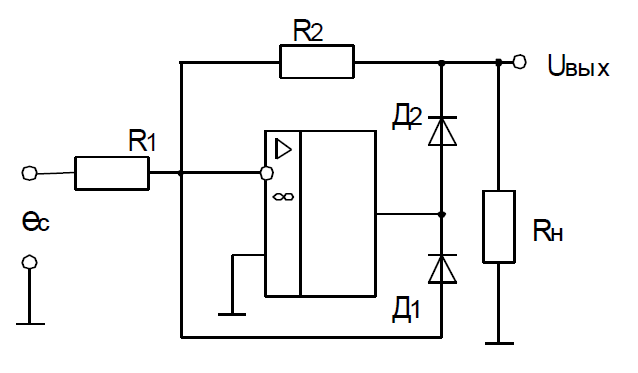
\includegraphics[scale=0.49]{scheme1}
		\caption{Выпрямитель, построенный \\на основе ОУ}
	\end{subfigure}
	\begin{subfigure}[b]{0.45\textwidth}
		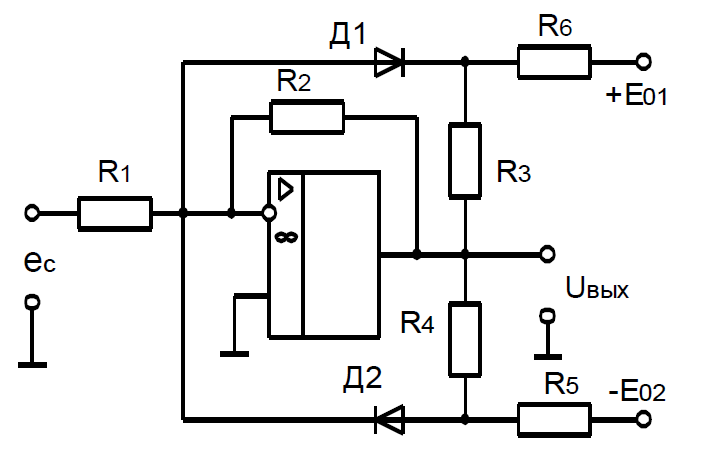
\includegraphics[scale=0.39]{scheme2}
		\caption{Двухсторонний усилитель-ограничитель}
	\end{subfigure}
	\caption{}
\end{center}
\end{figure}


\section{Исходные данные}

Операционный усилитель \verb+К140УД6+.

\begin{table}[H]
\begin{center}
	\caption{Исходные данные}
	\def\tabcolsep{6pt}
	\begin{tabular}{|c|c|c|c|c|c|c|c|c|c|}
		\hline
		$U_\text{вых}$, В &
		$e_c$, В &
		$K1$ &
		$K2$ &
		$K3$ &
		$U_\text{огр}$, В &
		$R_1$, кОм &
		$R_{\text{н}}$, кОм &
		$E_{01}$, В &
		$E_{02}$, В \\
		\hline
		$\pm12$ &
		15 &
		10 &
		1 &
		2 &
		$\pm2$ &
		20 &
		10 &
		15 &
		15 \\
	    \hline	
	\end{tabular}
\end{center}
\end{table}

\section{Теоретические расчёты}

\subsection{Расчет параметров элементов}

\begin{equation}
	\label{eq:4:1}
	R_2 = K_1 \cdot R_1 = 10 \cdot 20 = 200 \text{ кОм}
\end{equation}

\begin{equation}
	\label{eq:4:2}
	R_3 = \frac{K_2 \cdot R_2}{K_1 - K_2} = \frac{1 \cdot 200}{10 - 1} = \frac{200}{9} = 22.2 \text{ кОм}
\end{equation}

\begin{equation}
	\label{eq:4:3}
	R_4 = \frac{K_3 \cdot R_2}{K_1 - K_3} = \frac{2 \cdot 200}{10 - 2} = \frac{400}{8} = 50 \text{ кОм}
\end{equation}

\begin{equation}
	\label{eq:4:4}
	R_5 = \frac{R_4 \cdot E_{02}}{U_{\text{огр}^{+}}} = \frac{50 \cdot 15}{2} = \frac{750}{2} = 375 \text{ кОм}
\end{equation}


\begin{equation}
	\label{eq:4:5}
	R_6 = -\frac{R_3 \cdot E_{01}}{U_{\text{огр}^{-}}} = -\frac{22.2 \cdot 15}{-2} = \frac{333}{2} = 166.5 \text{ кОм}
\end{equation}

\section{Экспериментально снятые зависимости}

\subsection{Выпрямитель}

\begin{table}[H]
\begin{center}
	\caption{Зависимость напряжения $U_\text{вых}$ от $U_\text{вх}$ выпрямителя}
	\label{tab:rectifier}
	\def\tabcolsep{30pt}
	\fontsize{13}{14}\selectfont
	\pgfplotstabletypeset[col sep=comma,
	    columns={u_in,u_out,k,u_out_t},
	    column type/.add={|c|}{},
	    columns/u_in/.style={fixed, precision=3, zerofill, column name={$U_\text{вх}$, В}},
	    columns/u_out/.style={fixed, precision=3, zerofill, column name={$U_\text{вых}$, В}},
	    columns/k/.style={fixed, precision=2, zerofill, column name={$K$}},,
	    columns/u_out_t/.style={fixed, precision=3, zerofill, column name={$U_\text{вых теор}$, В}},
	    every nth row={1}{before row=\hline},
	    every head row/.style={before row=\hline, after row=\hline},
	    every last row/.style={after row=\hline}
	   ]{data/scheme1.csv}
\end{center}
\end{table}

Вычислим значения $K_{1 \text{ эксп}}$ как среднее арифметическое экспериментально полученных значений:

\begin{displaymath}
	K_{1\text{ эксп}} = \frac{\sum_{i=1}^{17} K_i}{17} = \frac{177.07}{17} = 10.42
\end{displaymath}

\begin{figure}[H]
\begin{center}
	\begin{tikzpicture} [every plot/.append style={thick}]
		\begin{axis}[
			height=0.45\textheight,
			width=0.95\textwidth,
			legend pos = north east,
			xlabel={$U_\text{вх}$, В},
			ylabel={$U_\text{вых}$, В},
			axis x line = middle,
			axis y line = middle,
			xmin = 0,
			xmax = 1.8,
			ymin = 0,
			ymax = 18,
			grid=major
		]
		\addplot [mark=square*, blue] table[x=u_in,y=u_out,col sep=comma]{data/scheme1.csv};
		\addplot [mark=*, dashed, red] table[x=u_in,y=u_out_t,col sep=comma]{data/scheme1.csv};
		\legend{Эксп., Теор.}
		\end{axis}
	\end{tikzpicture}
	\caption{Зависимость напряжения $U_\text{вых}$ от $U_\text{вх}$}
	\label{plot:rectifier}
\end{center}
\end{figure}

\newpage

\subsection{Двухсторонний усилитель-ограничитель}

\begin{table}[H]
\begin{center}
	\caption{Зависимость напряжения $U_\text{вых}$ от $U_\text{вх}$ двухстороннего усилителя-ограничителя}
	\label{tab:limiter}
	\def\tabcolsep{20pt}
	\def\arraystretch{1.23}
	\fontsize{13}{14}\selectfont
	\pgfplotstabletypeset[col sep=comma,
	    columns={u_in,u_out,k,u_out_t,k_t},
	    column type/.add={|c|}{},
	    columns/u_in/.style={fixed, precision=3, zerofill, column name={$U_\text{вх}$, В}},
	    columns/u_out/.style={fixed, precision=3, zerofill, column name={$U_\text{вых}$, В}},
	    columns/k/.style={fixed, precision=2, zerofill, column name={$K$}},
	    columns/u_out_t/.style={fixed, precision=3, zerofill, column name={$U_\text{вых теор}$, В}},
	    columns/k_t/.style={fixed, precision=0, zerofill, column name={$K_\text{теор}$}},
	    every nth row={1}{before row=\hline},
	    every head row/.style={before row=\hline, after row=\hline},
	    every last row/.style={after row=\hline}
	   ]{data/scheme2.csv}
\end{center}
\end{table}

Вычислим значения $K_{1 \text{ эксп}}$, $K_{2 \text{ эксп}}$ и $K_{3 \text{ эксп}}$ как среднее арифметическое экспериментально полученных значений:

\begin{displaymath}
	K_{1 \text{ эксп}} = \frac{\sum_{i=1}^{6}K_i}{6} = \frac{58.12}{9.68} = 9.69
\end{displaymath}

\begin{displaymath}
	K_{2 \text{ эксп}} = \frac{\sum_{i=1}^{9}K_i}{9} = \frac{8.26}{9} = 0.92
\end{displaymath}

\begin{displaymath}
	K_{3 \text{ эксп}} = \frac{\sum_{i=1}^{10}K_i}{10} = \frac{19.48}{10} = 1.95
\end{displaymath}

На рисунке \ref{fig:oscillogram} изображена осциллограмма двухстороннего усилителя-ограничителя.

\begin{figure}[H]
\begin{center}
	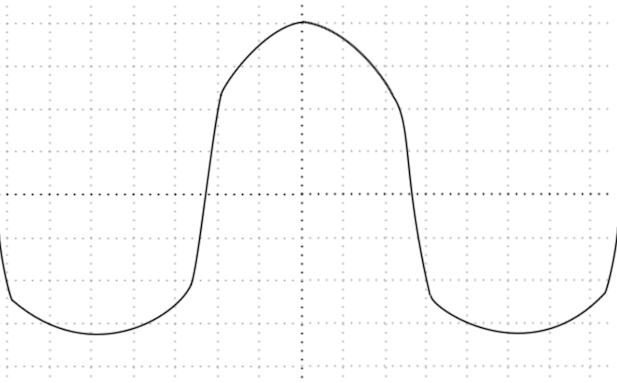
\includegraphics[scale=0.52]{curve}
	\caption{Осциллограмма двухстороннего усилителя-ограничителя, при этом \textbf{одно вертикальное деление равняется 1 Вольту}}
	\label{fig:oscillogram}
\end{center}
\end{figure}

На рисунке \ref{plot:limiter} изображен общий вид зависимости напряжения $U_\text{вых}$ от $U_\text{вх}$ двухстороннего усилителя-ограничителя. На рисунке \ref{plot:limiter_detail} изображена та же зависимость в области $|U_\text{вых}| \le U_\text{огр}$.

\begin{figure}[H]
\begin{center}
	\begin{tikzpicture} [every plot/.append style={thick}]
		\begin{axis}[
			height=0.45\textheight,
			width=0.95\textwidth,
			legend pos = north east,
			xlabel={$U_\text{вх}$, В},
			ylabel={$U_\text{вых}$, В},
			axis x line = middle,
			axis y line = middle,
			xmin = -8,
			xmax = 14,
			ymin = -15,
			ymax = 15,
			grid=major
		]
		\addplot table[x=u_in,y=u_out,col sep=comma]{data/scheme2.csv};
		\addplot table[x=u_in,y=u_out_t,col sep=comma]{data/scheme2.csv};
		\legend{Эксп., Теор.}
		\end{axis}
	\end{tikzpicture}
	\caption{Общий вид зависимости напряжения $U_\text{вых}$ от $U_\text{вх}$}
	\label{plot:limiter}
\end{center}
\end{figure}

\vspace{-1.1cm}

\begin{figure}[H]
\begin{center}
	\begin{tikzpicture} [every plot/.append style={thick}]
		\begin{axis}[
			x tick label style={
				/pgf/number format/.cd,
				fixed,
				precision=2,
				/tikz/.cd
			},
			height=0.45\textheight,
			width=0.95\textwidth,
			legend pos = north east,
			xlabel={$U_\text{вх}$, В},
			ylabel={$U_\text{вых}$, В},
			axis x line = middle,
			axis y line = middle,
			xmin = -0.25,
			xmax = 0.25,
			ymin = -2.5,
			ymax = 2.5,
			grid=major
		]
		\addplot table[x=u_in,y=u_out,col sep=comma]{data/scheme2.csv};
		\addplot table[x=u_in,y=u_out_t,col sep=comma]{data/scheme2.csv};
		\draw[black,very thick,dashed] (axis cs:0,2.3) -- (axis cs:-0.23,2.3) -- (axis cs:-0.23,0);
		\draw[black,very thick,dashed] (axis cs:0,-2.2) -- (axis cs:0.22,-2.2) -- (axis cs:0.22,0);
		\legend{Эксп., Теор.}
		\end{axis}
	\end{tikzpicture}
	\caption{Зависимость напряжения $U_\text{вых}$ от $U_\text{вх}$ в области $|U_\text{вых}| \le U_\text{огр}$}
	\label{plot:limiter_detail}
\end{center}
\end{figure}

\section{Погрешности}

\subsection{Выпрямитель}

\begin{displaymath}
	\delta_{max} K_1 = \sqrt{(\delta R_1)^2 + (\delta R_2)^2} = \sqrt{0.1^2 + 0.1^2} = 0.141 = 14.1 \%
\end{displaymath}

\begin{displaymath}
	\delta K_1 = \left| \frac{K_{1 \text{ теор.}} - K_{1 \text{ эксп.}}}{K_{1 \text{ теор.}}} \right| = \left| \frac{10 - 10.42}{10} \right| = 0.042 = 4.2 \% < \delta_{max} K_1 = 14.1 \%
\end{displaymath}

\subsection{Двухсторонний усилитель-ограничитель}

\begin{displaymath}
	\delta_{max} K_1 = \sqrt{(\delta R_1)^2 + (\delta R_2)^2} = \sqrt{0.1^2 + 0.1^2} = 0.141 = 14.1 \%
\end{displaymath}

\begin{displaymath}
	\delta_{max} K_{2} = \sqrt{(\delta R_1)^2 + (\delta R_2)^2 + (\delta R_3)^2 + (\delta R_6)^2} = \sqrt{4 \cdot 0.1^2} = 0.2 = 20 \%
\end{displaymath}

\begin{displaymath}
	\delta_{max} K_{3} = \sqrt{(\delta R_1)^2 + (\delta R_2)^2 + (\delta R_4)^2 + (\delta R_5)^2} = \sqrt{4 \cdot 0.1^2} = 0.2 = 20 \%
\end{displaymath}

\begin{displaymath}
	\delta K_1 = \left| \frac{K_{1 \text{ теор.}} - K_{1 \text{ эксп.}}}{K_{1 \text{ теор.}}} \right| = \left| \frac{10 - 9.69}{10} \right| = 0.031 = 3.1 \% < \delta_{max} K_{1} = 14.1 \%
\end{displaymath}

\begin{displaymath}
	\delta K_2 = \left| \frac{K_{2 \text{ теор.}} - K_{2 \text{ эксп.}}}{K_{2 \text{ теор.}}} \right| = \left| \frac{1 - 0.92}{1} \right| = 0.08 = 8 \% < \delta_{max} K_{2} = 20 \%
\end{displaymath}

\begin{displaymath}
	\delta K_3 = \left| \frac{K_{3 \text{ теор.}} - K_{3 \text{ эксп.}}}{K_{3 \text{ теор.}}} \right| = \left| \frac{2 - 1.95}{2} \right| = 0.025 = 2.5 \% < \delta_{max} K_{3} = 20 \%
\end{displaymath}

\section{Выводы}

Приведённые погрешности полученных в ходе эксперимента значений $K_1$, $K_2$ и $K_3$ не превышают предельно допустимые погрешности.

Таким образом, формулы \ref{eq:4:1} -- \ref{eq:4:5} являются верными.

\end{document}